\documentclass{beamer}

\usepackage[utf8]{inputenc}
\usepackage{hyperref}

\usetheme{Berkeley}
\beamertemplatenavigationsymbolsempty
\setbeamertemplate{headline}{}
 
\title{Including data in FoodChain-Lab}
\date{}
 
\begin{document}
\maketitle

\section{ }

\subsection{Tasks}
\begin{frame}
	\begin{itemize}
		\item Import the following file into a an empty database: \url{https://github.com/SiLeBAT/BfROpenLabResources/raw/master/GitHubPages/documents/1_Lieferliste Caterer 1a.xlsx}
		\item Generate a new template for data import in order to add missing data.
        \item Fill in the template.
        \item Import new data into the database.
	\end{itemize}
\end{frame}
 
\subsection{1}
\begin{frame}
	\begin{center}
  		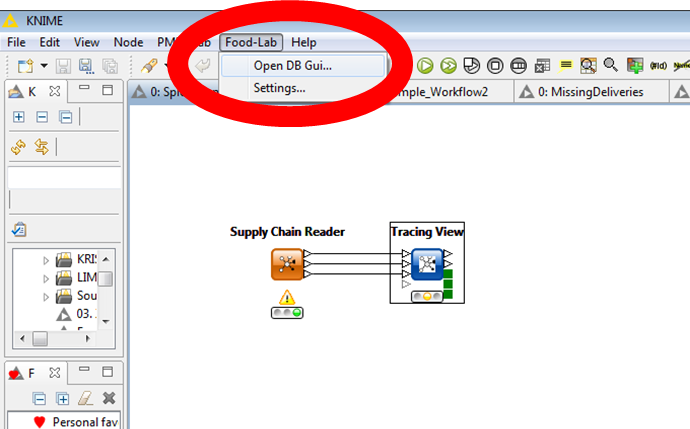
\includegraphics[height=0.6\textheight]{1.png}
	\end{center}
	\begin{itemize}
		\item Open the database window via the \textbf{KNIME} menu \textbf{Food-Lab $>$ Open DB Gui...}.
	\end{itemize}
\end{frame}

\subsection{2}
\begin{frame}
	\begin{center}
  		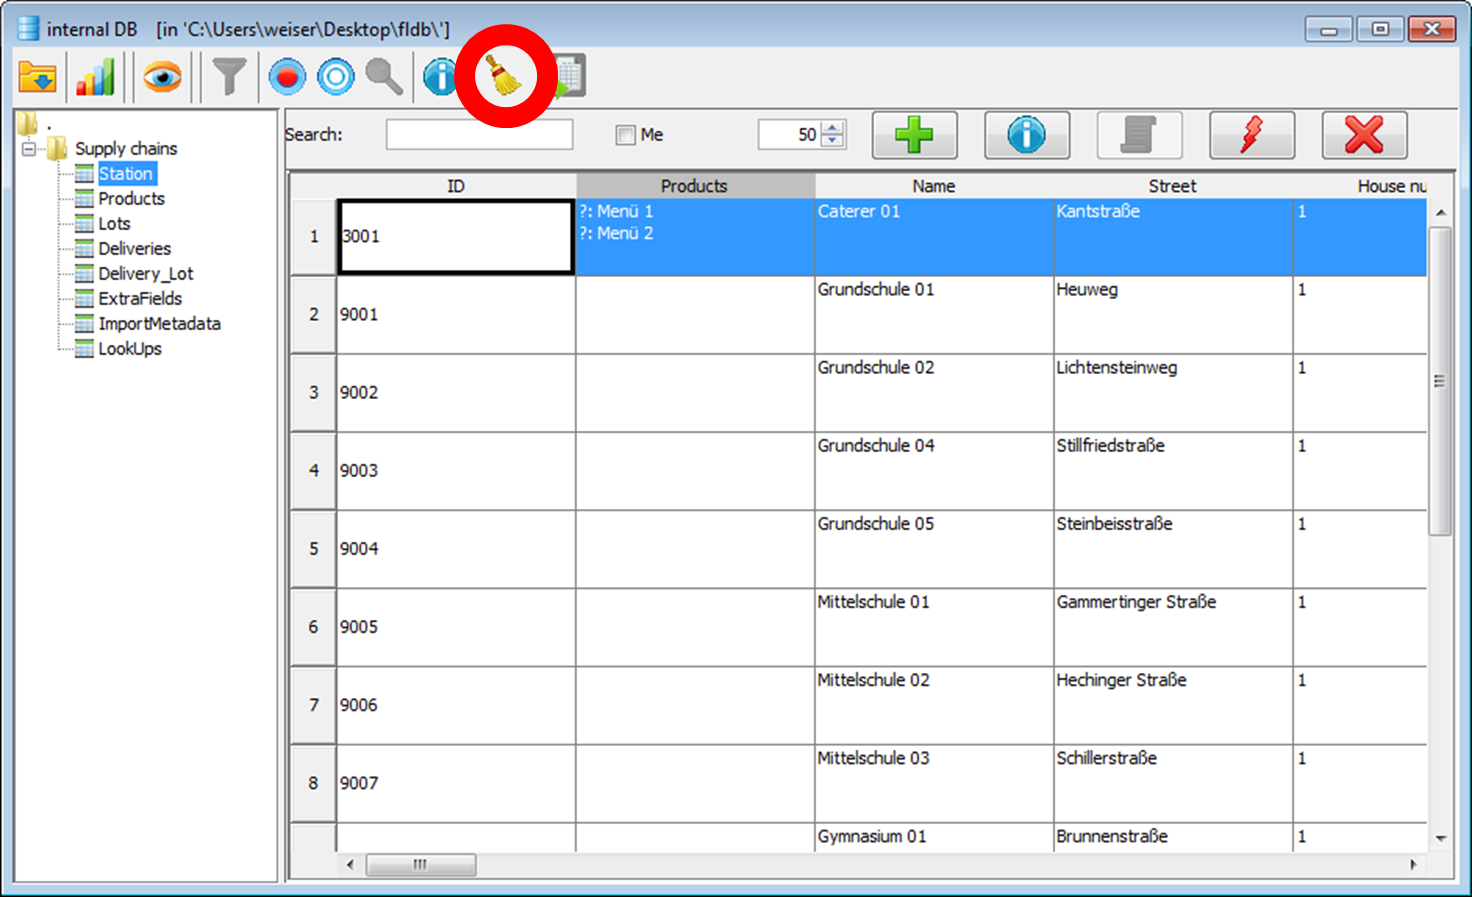
\includegraphics[height=0.6\textheight]{2.png}
	\end{center}
	\begin{itemize}
		\item The database window opens.
		\item Click the broom symbol in the toolbar to reset the database. Cauton: All entries in the local database are going to be deleted! A new and empty database is going to be generated.
		\item Before setting up a new database you can produce a data backup with the red button in the toolbar.
	\end{itemize}
\end{frame}

\subsection{3}
\begin{frame}
	\begin{center}
  		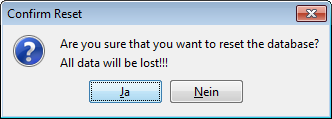
\includegraphics[height=0.3\textheight]{3.png}
	\end{center}
	\begin{itemize}
		\item Confirm the database reset with \textbf{Ja}.
	\end{itemize}
\end{frame}

\subsection{4}
\begin{frame}
	\begin{center}
  		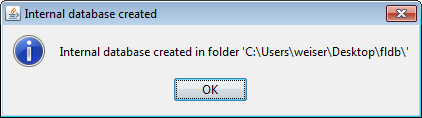
\includegraphics[width=0.9\textwidth]{4.png}
	\end{center}
	\begin{itemize}
		\item The database window closes and the following dialog appears.
		\item Acknowledge the dialog with \textbf{OK}. Afterwards, the database window opens again and all tables are empty.
	\end{itemize}
\end{frame}

\subsection{5}
\begin{frame}
	\begin{center}
  		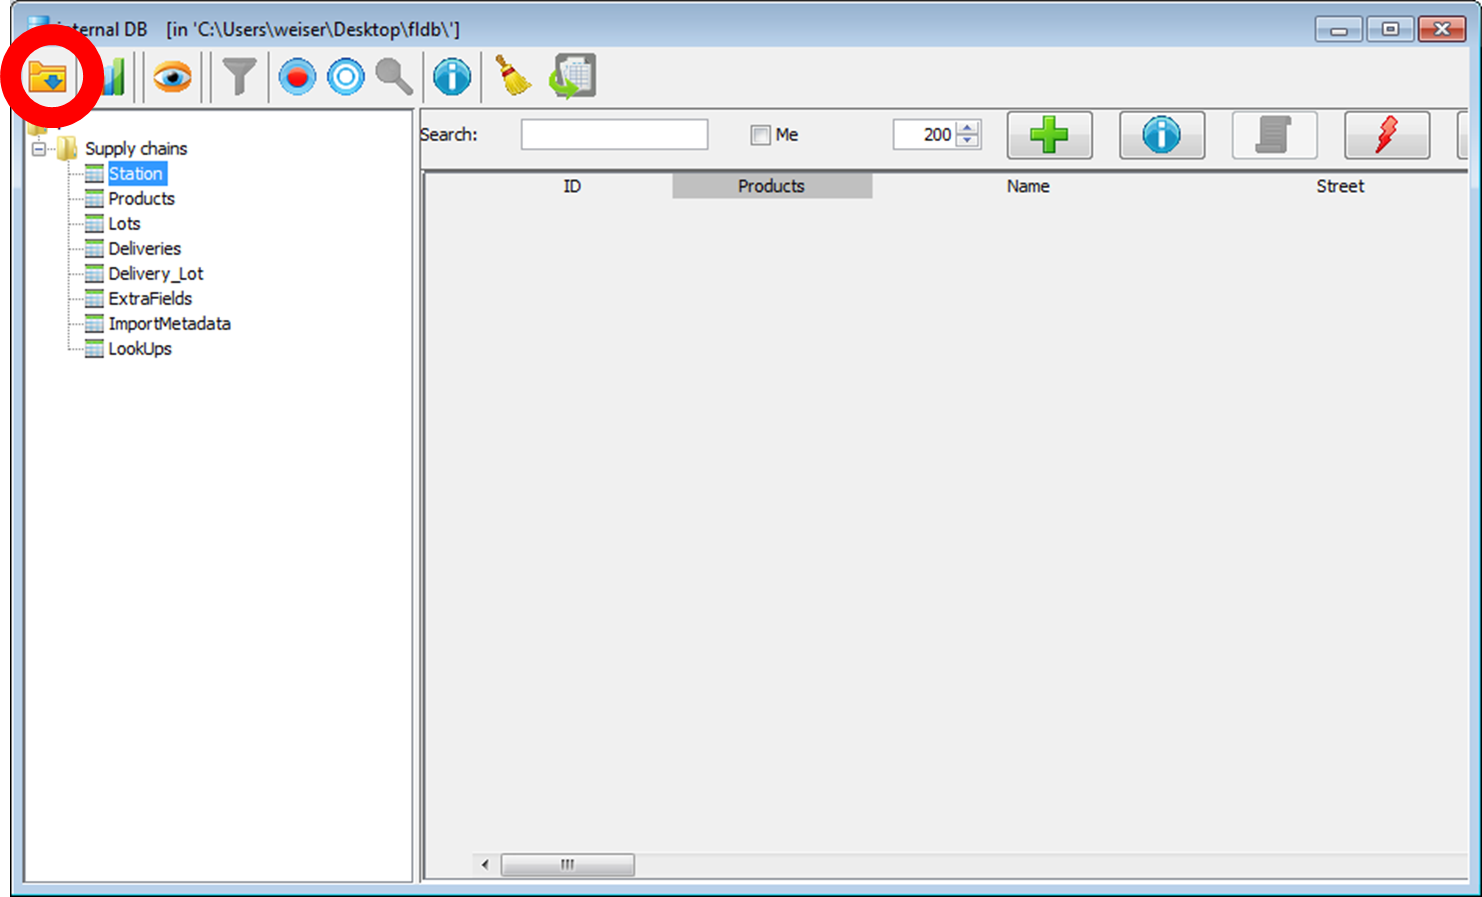
\includegraphics[width=0.9\textwidth]{5.png}
	\end{center}
	\begin{itemize}
		\item Click the folder symbol with the blue arrow to open the import dialog.
	\end{itemize}
\end{frame}

\subsection{6}
\begin{frame}
	\begin{center}
  		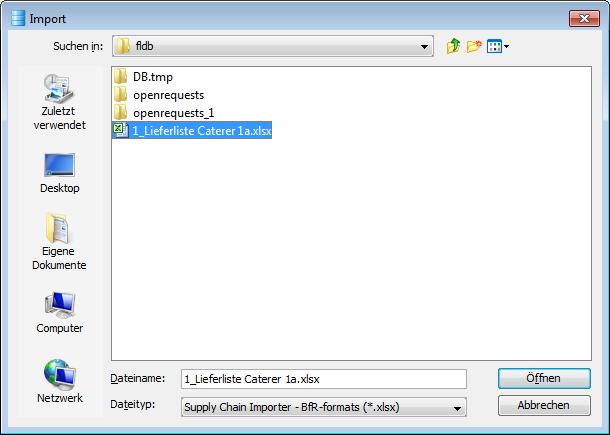
\includegraphics[height=0.6\textheight]{6.png}
	\end{center}
	\begin{itemize}
		\item In the import dialog choose the Excel file you can download from  \url{https://github.com/SiLeBAT/BfROpenLabResources/raw/master/GitHubPages/documents/1_Lieferliste Caterer 1a.xlsx}.
		\item Click \textbf{Öffnen}.
	\end{itemize}
\end{frame}

\subsection{7}
\begin{frame}
	\begin{center}
  		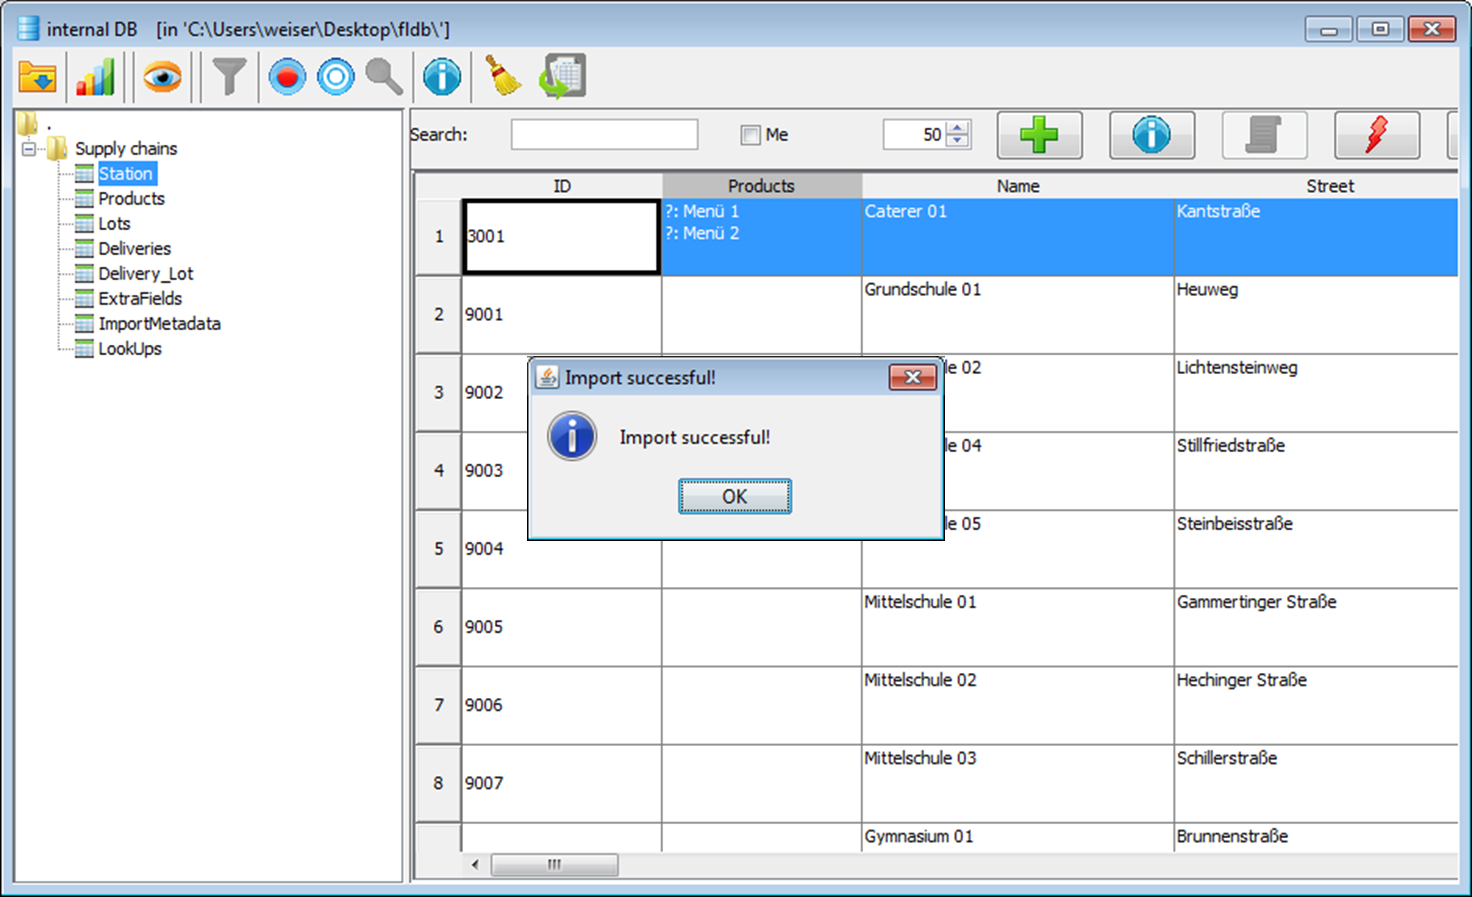
\includegraphics[height=0.6\textheight]{7.png}
	\end{center}
	\begin{itemize}
		\item The tables in the database have been supplemented.
		\item The successful import is stated in a small window.
        \item Close this window by clicking \textbf{OK}.
        \item You can have a look at the imported data, for example with the TracingView (see subsection 8 in the tutorial \url{http://foodrisklabs.bfr.bund.de/index.php/erstellen-eines-workflow-in-foodchain-lab-teil-1/} and in \url{http://foodrisklabs.bfr.bund.de/index.php/erstellen-eines-workflows-in-foodchain-lab-teil-2/}.
	\end{itemize}
\end{frame}

\subsection{8}
\begin{frame}
	\begin{center}
  		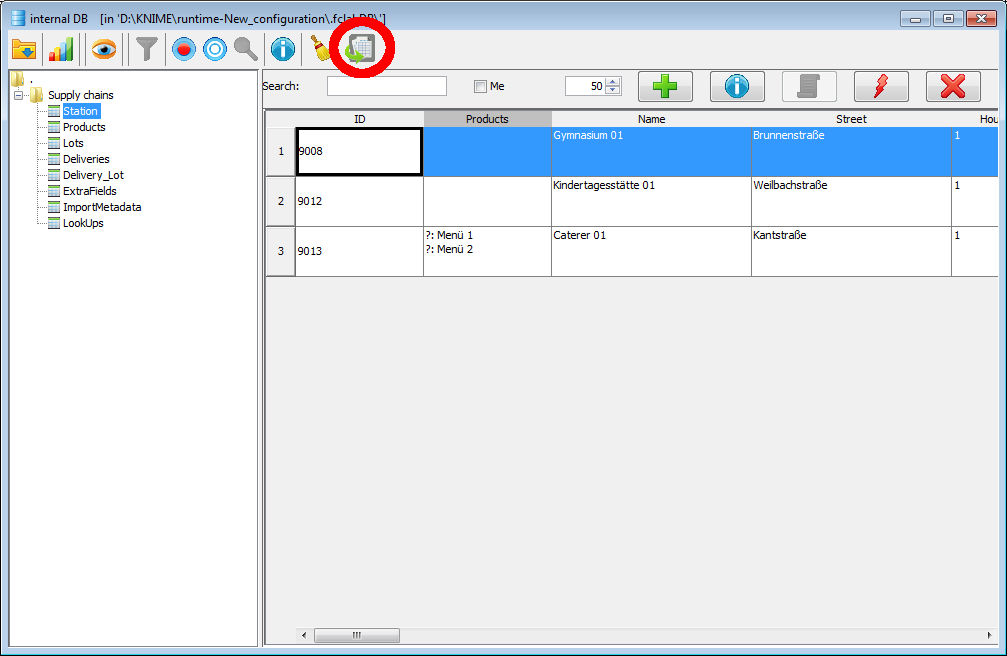
\includegraphics[width=0.7\textwidth]{8.png}
	\end{center}
	\begin{itemize}
		\item Click the symbol in the toolbar representing a table with a curved green arrow directing to the left hand side.
	\end{itemize}
\end{frame}

\subsection{9}
\begin{frame}
	\begin{center}
  		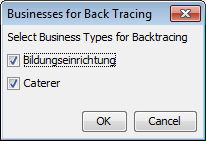
\includegraphics[height=0.5\textheight]{9.png}
	\end{center}
	\begin{itemize}
		\item A dialog opens enabling you to select the businesses for back-tracing.
		\item Confirm your selection with \textbf{OK}.
	\end{itemize}
\end{frame}

\subsection{10}
\begin{frame}
	\begin{center}
  		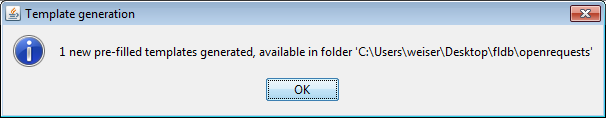
\includegraphics[height=0.2\textheight]{10.png}
	\end{center}
	\begin{itemize}
		\item A window opens to define a folder for saving templates. Select a folder or create a new one and click \textbf{Open}.
		\item The database is checked for missing information and templates optimised for data acquisition are generated.
		\item Click \textbf{OK} to close the window informing about the successful template generation.
	\end{itemize}
\end{frame}

\subsection{11}
\begin{frame}
	\begin{center}
  		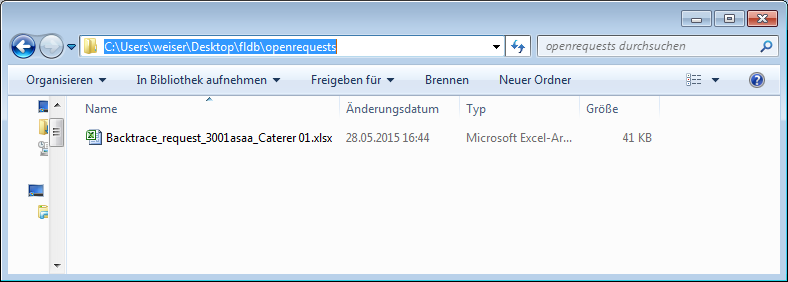
\includegraphics[height=0.4\textheight]{11.png}
	\end{center} 	
	\begin{itemize}
		\item Open the generated template by double-clicking the symbol in your file manager.
		\item The file can be edited with Microsoft Excel or LibreOffice.
	\end{itemize}
\end{frame}

\subsection{12}
\begin{frame}
	\begin{center}
  		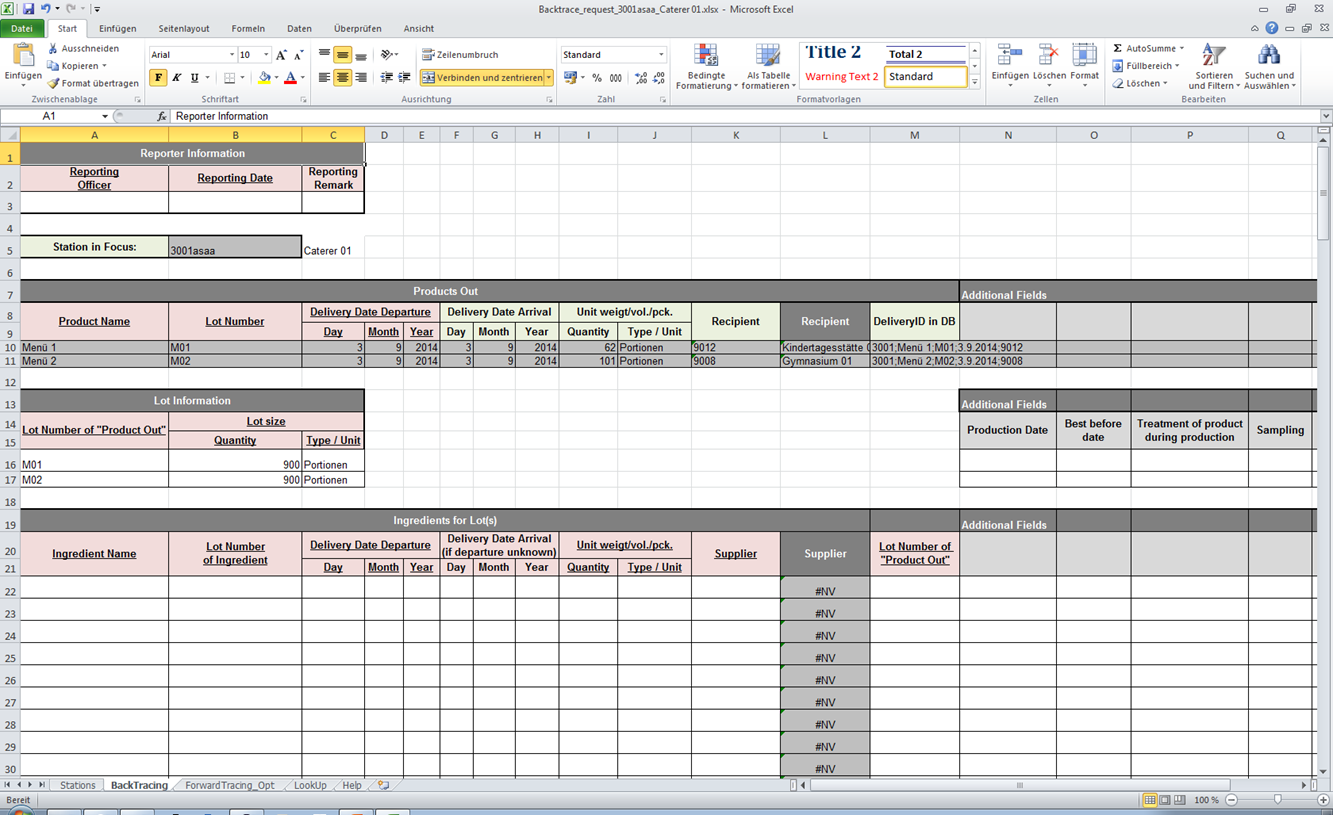
\includegraphics[height=0.5\textheight]{12.png}
	\end{center}
	\begin{itemize}
		\item The Excel file consists of several sheets.
		\item Important for editing are the sheets \textbf{Stations}, \textbf{BackTracing}and \textbf{LookUp}
		\item The screenshot shows the sheet \textbf{BackTracing}, in which several deliveries have been entered automatically based on database entries.
		\item The template is needed to collect information about ingredients and their suppliers in order to be able to understand (and to visualise in FoodChain-Lab) the delivery network.
		\item Information needs to be added or corrected in cells below headlines highlighted in light red.
	\end{itemize}
\end{frame}

\subsection{13}
\begin{frame}
	\begin{center}
  		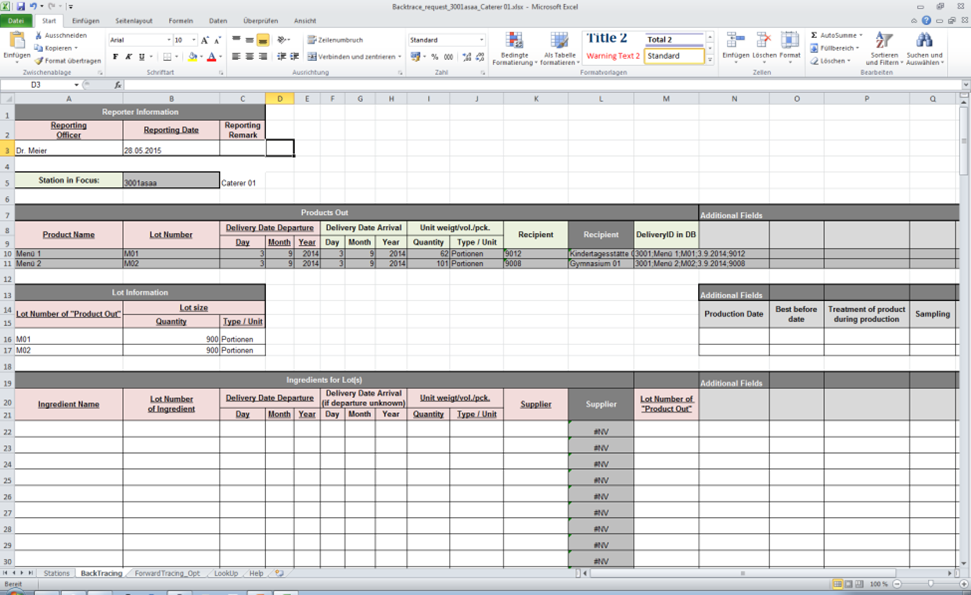
\includegraphics[height=0.65\textheight]{13.png}
	\end{center}
	\begin{itemize}
		\item Enter in line 3 the name of the reporting officer.
		\item Line 5 informs about the station in focus, which is in this case a caterer. 
		\item Lines 7 to 11 show the deliveries for which the utilised ingredients need to be added.
	\end{itemize}
\end{frame}

\subsection{14}
\begin{frame}
	\begin{center}
  		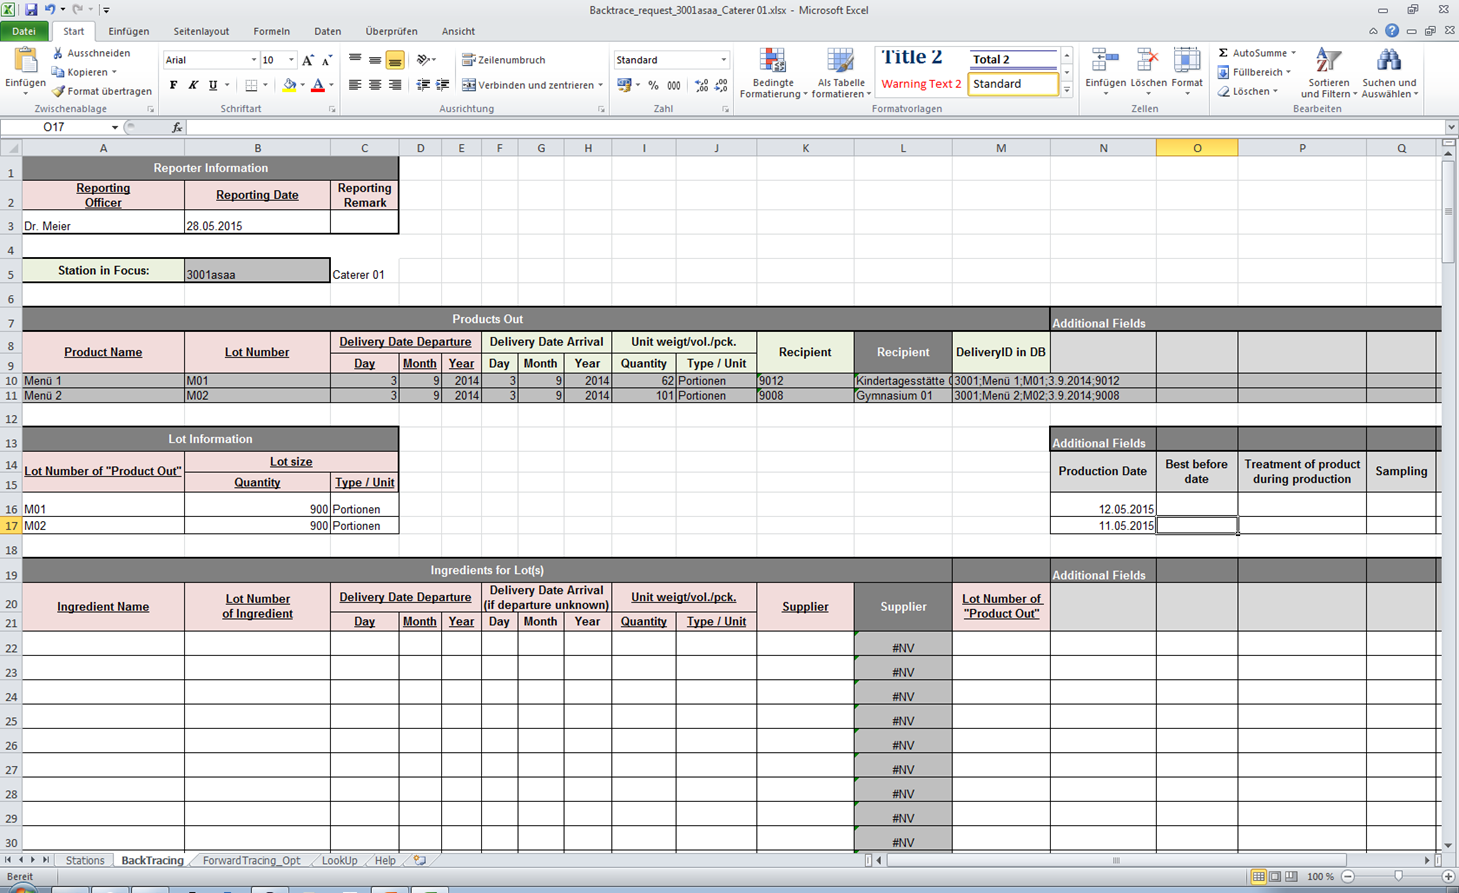
\includegraphics[height=0.6\textheight]{14.png}
	\end{center}
	\begin{itemize}
		\item In this case the \textbf{Lot size} is already known meaning that in lines 13 to 17 no information needs to be added. However, in case of wrong database entries the uncoloured lines (lines 16 and 17) should be corrected.
		\item It is possible to define \textbf{Additional Fields}, for example to state the \textbf{Production Date}.
	\end{itemize}
\end{frame}

\subsection{15}
\begin{frame}
	\begin{center}
  		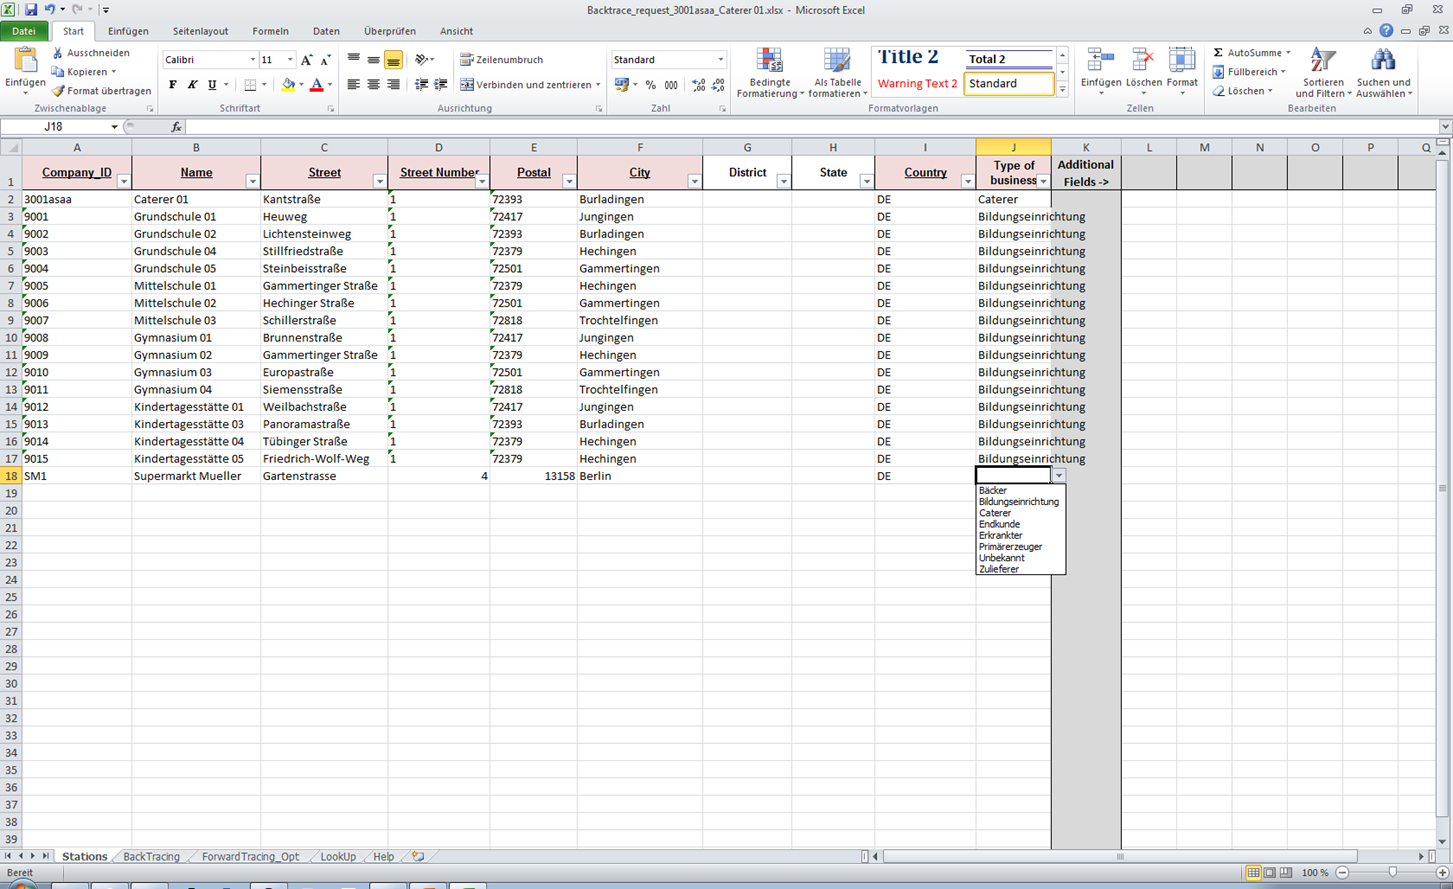
\includegraphics[height=0.6\textheight]{15.png}
	\end{center}
	\begin{itemize}
		\item New stations (e.g. a food producer or a supermarket) can be defined in the sheet \textbf{Stations}.
		\item Define the new station \textbf{Supermarkt Mueller} (a supermarket).
		\item The \textbf{Type of business} for the new station is '\textbf{Zulieferer}' (meaning 'supplier').
	\end{itemize}
\end{frame}

\subsection{16}
\begin{frame}
	\begin{center}
  		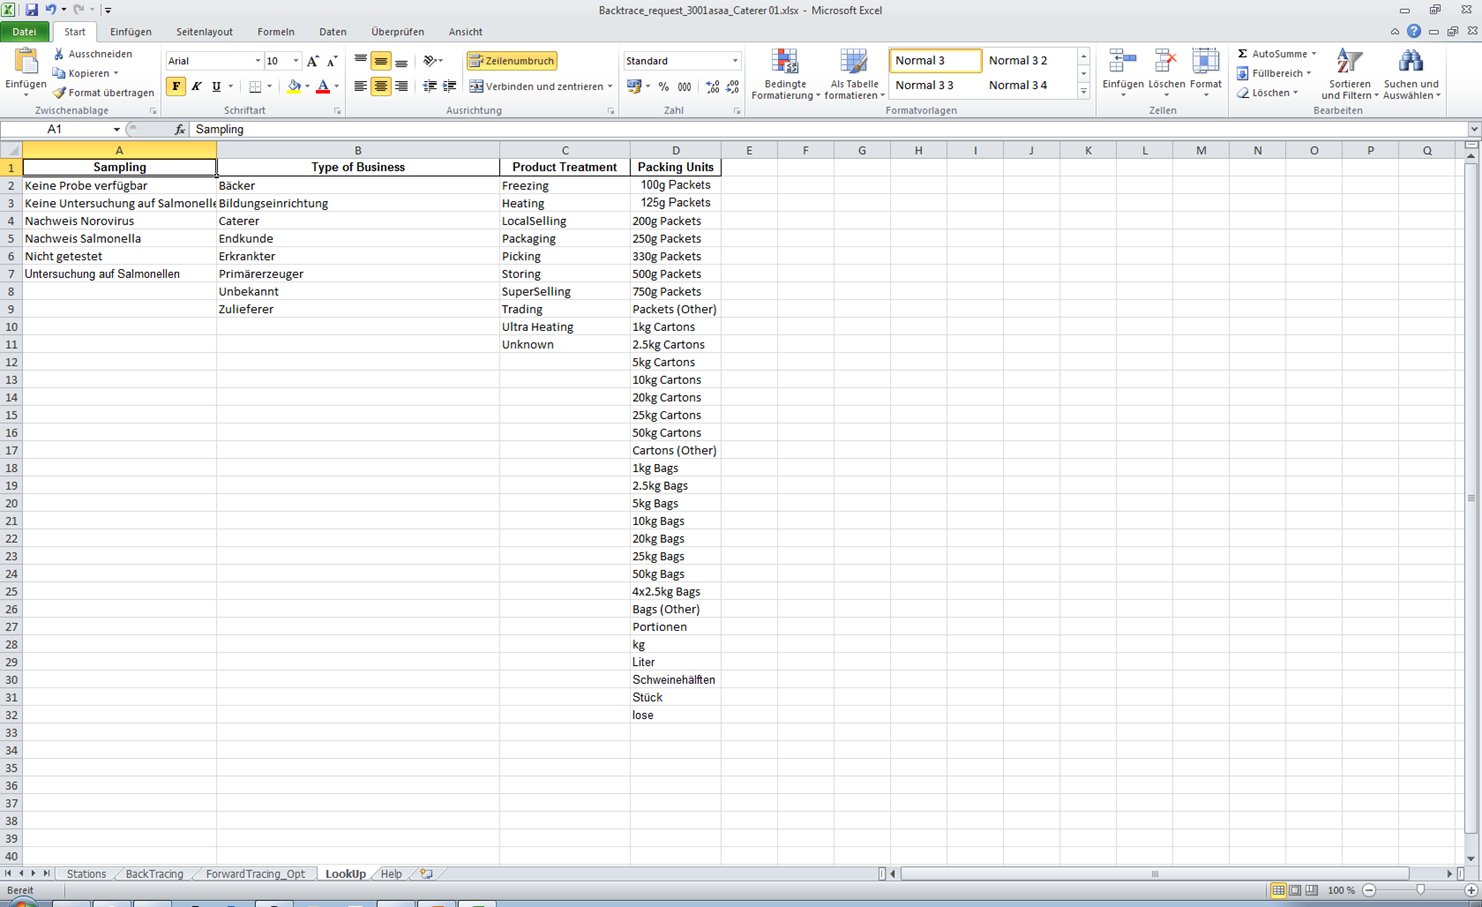
\includegraphics[height=0.6\textheight]{16.png}
	\end{center}
	\begin{itemize}
		\item The whole list of choices for \textbf{Type of business} can be viewed in the sheet \textbf{LookUp}.
		\item In the look-up table sampling information, the type of business, product treatment information and packing units can be corrected or created.
		\item Changes in the look-up table should be agreed on with the main data manager.
	\end{itemize}
\end{frame}

\subsection{17}
\begin{frame}
	\begin{center}
  		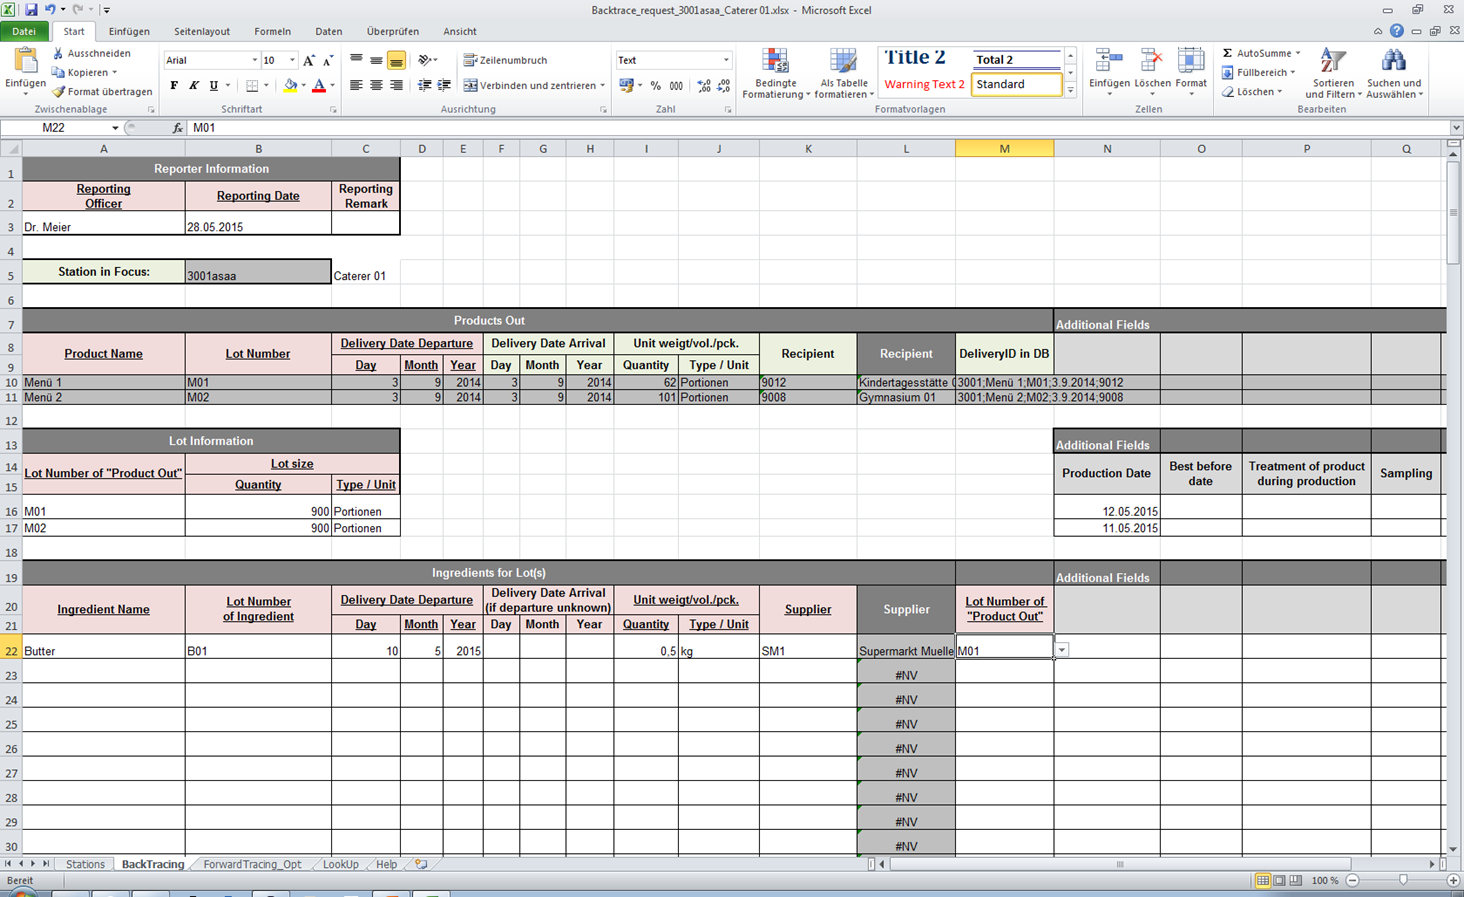
\includegraphics[height=0.6\textheight]{17.png}
	\end{center}
	\begin{itemize}
		\item In the sheet \textbf{BackTracing} the ingredients of the two deliveries or lot numbers (see lines 10/11 or 16/17) should be entered.
		\item To do this please fill in the lines from line 22.
	\end{itemize}
\end{frame}

\subsection{18}
\begin{frame}
	\begin{center}
  		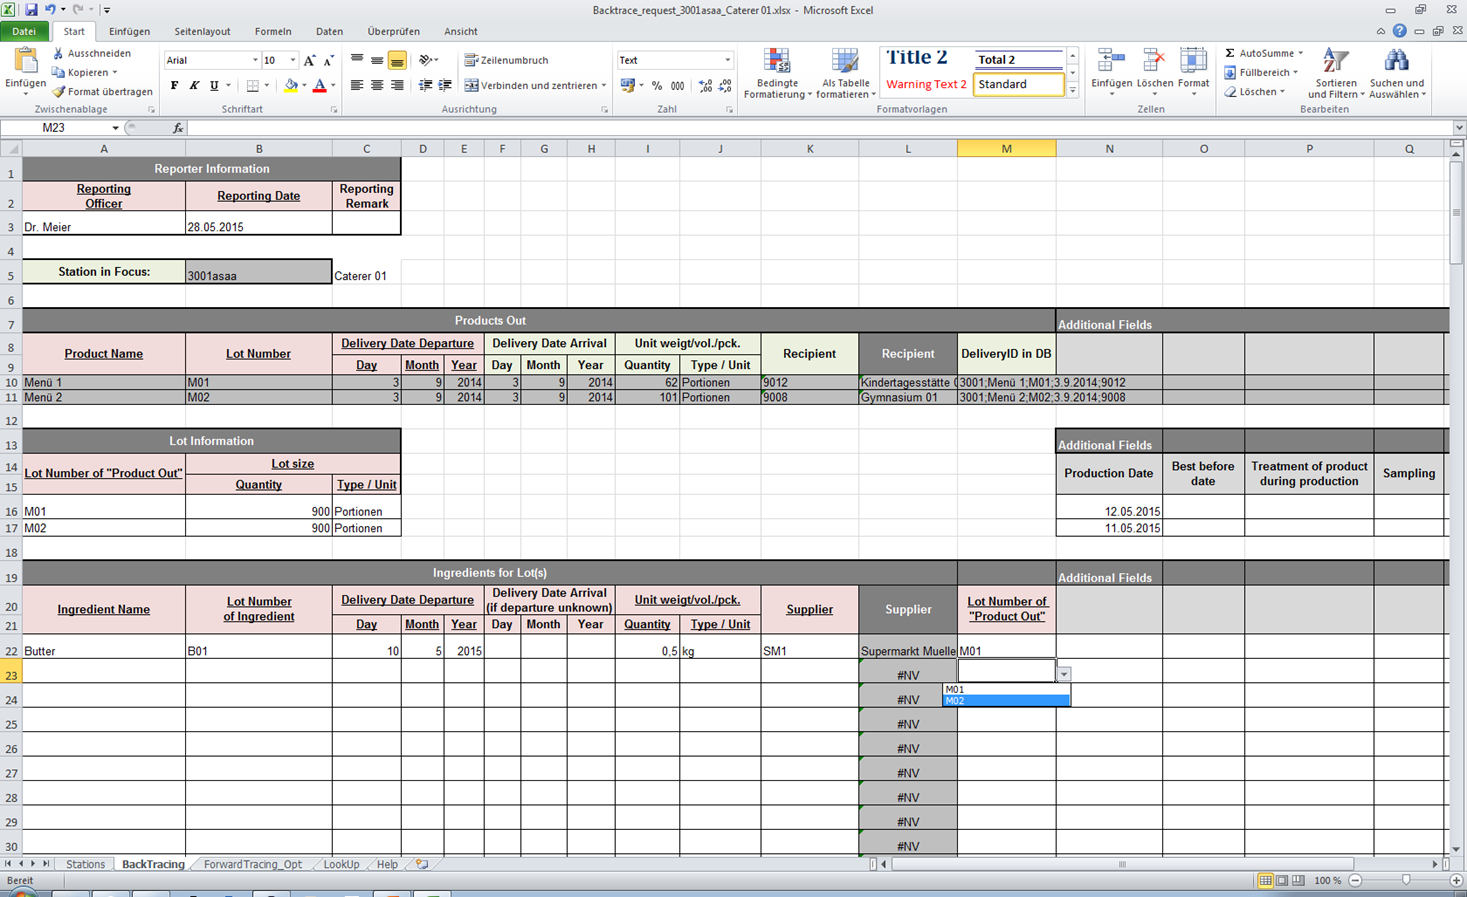
\includegraphics[height=0.6\textheight]{18.png}
	\end{center}
	\begin{itemize}
		\item Please choose for every delivery the appropriate lot number (column M) from the drop-down list.
	\end{itemize}
\end{frame}

\subsection{19}
\begin{frame}
	\begin{center}
  		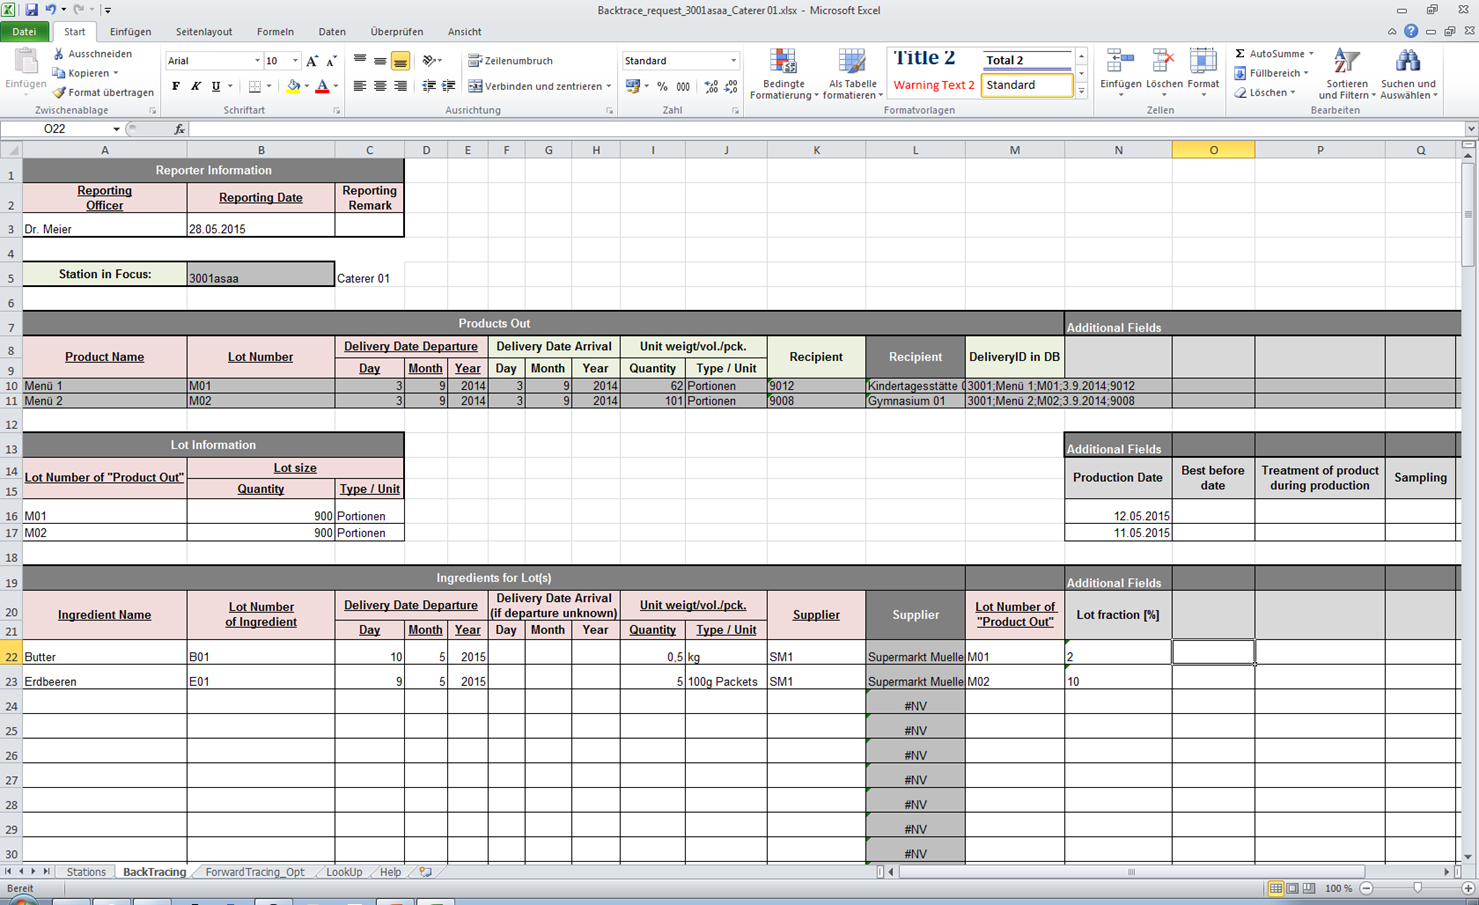
\includegraphics[height=0.6\textheight]{19.png}
	\end{center}
	\begin{itemize}
		\item Here, it is also possible to define \textbf{Additional Fields} to collect additional data, for example as shown here for \textbf{Lot fraction [\%]}.
		\item Afterwards, this information is also available for analyses in FoodChain-Lab.
		\item Usually the main data manager defines additional fields in advance.
	\end{itemize}
\end{frame}

\subsection{20}
\begin{frame}
	\begin{center}
  		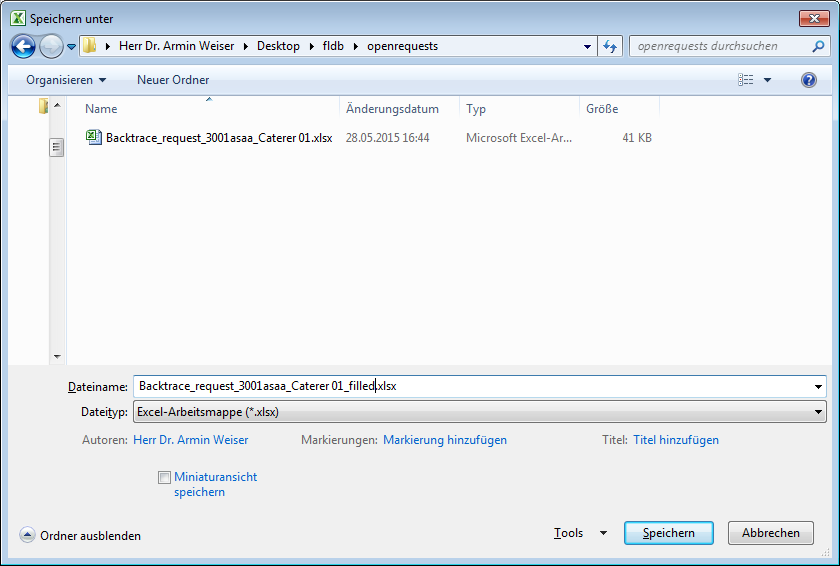
\includegraphics[height=0.6\textheight]{20.png}
	\end{center}
	\begin{itemize}
		\item Save the edited template.
	\end{itemize}
\end{frame}


\subsection{21}
\begin{frame}
	\begin{center}
  		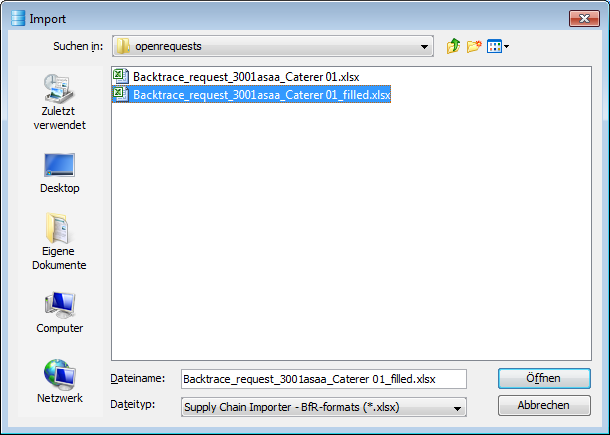
\includegraphics[height=0.6\textheight]{21.png}
	\end{center}
	\begin{itemize}
		\item Go back to the database window in FoodChain-Lab or open it again via \textbf{Food-Lab $>$ Open DB Gui...}.
		\item Click the folder symbol with the blue arrow.
		\item The import dialog opens.
		\item Choose the edited backtracing template file.
		\item Click \textbf{Öffnen}.
	\end{itemize}
\end{frame}

\subsection{22}
\begin{frame}
	\begin{center}
  		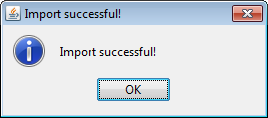
\includegraphics[height=0.3\textheight]{22.png}
	\end{center}
	\begin{itemize}
		\item Information has been added to the database tables.
		\item The successful import is stated in a small window.
		\item Click \textbf{OK} to close the window.
		\item Data can now be analysed with FoodChain-Lab analysieren. Please use the respective tutorials as needed.
	\end{itemize}
\end{frame}

\end{document}